\documentclass[tikz,border=5pt]{standalone}
\usepackage{amsmath,amssymb}
\usetikzlibrary{arrows.meta}
\definecolor{addmass}{RGB}{30,95,150}
\definecolor{removemass}{RGB}{175,60,45}
\tikzset{source/.style={circle,draw=black,fill=white,inner sep=2pt,minimum size=6pt},target/.style={rectangle,draw=black,fill=white,inner sep=2pt,minimum size=6pt},add/.style={-{Stealth[length=2mm]},thick,draw=addmass},remove/.style={-{Stealth[length=2mm]},thick,dashed,draw=removemass},mass/.style={fill=white,inner sep=1pt,font=\small}}
\begin{document}
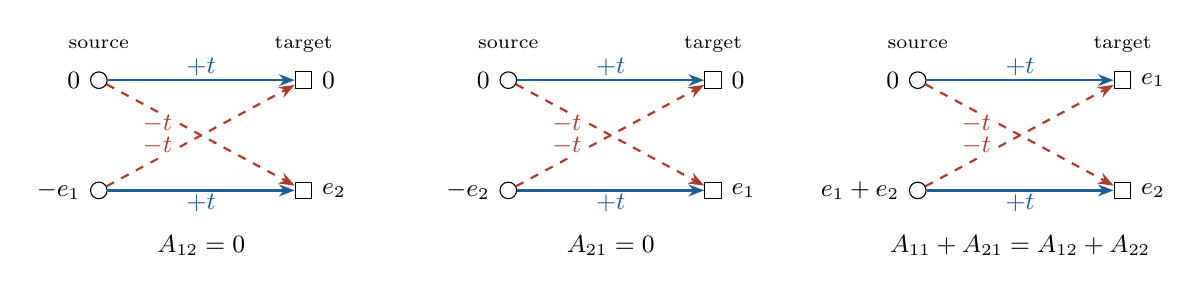
\begin{tikzpicture}[font=\small]
\foreach \shift/\sourcepoint/\targettop/\targetbottom/\condition in {
0/{-e_1}/{0}/{e_2}/{A_{12}=0},
5.2/{-e_2}/{0}/{e_1}/{A_{21}=0},
10.4/{e_1+e_2}/{e_1}/{e_2}/{A_{11}+A_{21}=A_{12}+A_{22}}}{
\begin{scope}[xshift=\shift cm]
\node[font=\scriptsize] at (0,2.25) {source};
\node[font=\scriptsize] at (2.6,2.25) {target};
\node[source,label=left:{$0$}] (s0) at (0,1.8) {};
\node[source,label=left:{$\sourcepoint$}] (s1) at (0,0.4) {};
\node[target,label=right:{$\targettop$}] (t0) at (2.6,1.8) {};
\node[target,label=right:{$\targetbottom$}] (t1) at (2.6,0.4) {};
\draw[add] (s0) -- node[mass,above,text=addmass] {$+t$} (t0);
\draw[add] (s1) -- node[mass,below,text=addmass] {$+t$} (t1);
\draw[remove] (s0) -- node[mass,pos=.27,below,text=removemass] {$-t$} (t1);
\draw[remove] (s1) -- node[mass,pos=.27,above,text=removemass] {$-t$} (t0);
\node at (1.3,-0.3) {$\condition$};
\end{scope}
}
\end{tikzpicture}
\end{document}
